%%
\subsection{Metamorphic Testing(MT)}

% FRAME
\begin{frame}[fragile]
	\frametitle{Metamorphic Testing(MT)}
	%% \structure{What is MT}
	\begin{itemize}
		\item comparing outputs of successive runs with varying(morphed) input data for validation
		\item Metamorphic Relation(MR): intrinsic function of software idetified for validating
	\end{itemize}	

			\begin{figure}
				 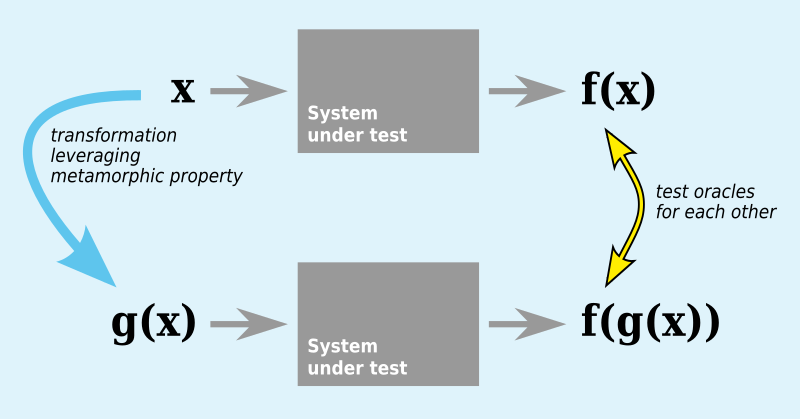
\includegraphics[scale = 0.30]{images/Metamorphic_Testing_image}
				%% \includegraphics[width = 0.95\textwidth]{images/Metamorphic testing.png}
				\linebreak
			 	\tiny{image:Metamorphic Testing by Teemu Kanstrén from Towards Data Science}
			\end{figure}
		
	
\end{frame}


%%%%%%%%%%%%%%%%%%%%%%%%%%%%%%%%%

% FRAME
\begin{frame}[fragile]
	\structure{ Metamorphic Relations}
		\begin{itemize}
			
			\item MRs are usually identified based on the system under test by domain experts
			\item Permutative(change the order of keywords in a search )
			\item Additive, Multiplicative (add or multiplying by a constant, resulting in increase/no effect on output)
			\item Invertive(changing the signs of each data point, resulting in negative of previous output)
			\item Inclusive(adding a new constraint in the search criteria)
			\item Exclusive(removing elements from the data points)
			\item periodicity(explored in Hands on session)
			\item could be linear or quadratic $$ \cos{(2x)} = 2{\cos} ^2  (x)   $$
		\end{itemize}		
	
\end{frame}